% !Mode:: "TeX:UTF-8"
\chapter{FAT32文件系统卷的FAT数据结构}

所有FAT文件系统最初都是为IBM PC机器架构开发的,因此FAT对BPB,FAT和文件和目录条目中的条目使用小端格式[1]。 FAT数据结构是存储关于使用哪些集群,空闲或可能不可用的信息的表。除此之外,它还存储有关属于特定文件的集群链的信息。根据所使用的FAT文件系统的类型和卷的大小,簇大小会有所不同,每个簇的连续扇区数可能是1,2,4,8,16,32或64 [1]。由于每个容量的内存成本每年都在急剧下降[9],最大集群数量急剧增加,因此用于标识每个集群的位数也在增长。因此,FAT格式的连续主要版本以用于寻址集群的表元素位数来命名:12,16,32和64 [2]。在FAT32中,FAT条目是32位宽,但只有低28位用于寻址
2 \^ 28个簇。因此,FAT32体积可以与((2\^28)*64)/2KB一样大,等于8TB。

\section{基本设计技术}
FAT32卷上的每个文件和目录(根目录除外)在其父目录中都有一个包含名称,属性,大小等的条目以及分配给它的32位宽的第一个簇号。 对应任何簇编号,FAT条目可以具有下面给出的某些允许值:

\begin{table}[htbp]
	\centering
	\caption[基本设计技术]{基本设计技术}
	\begin{tabular}{lp{7cm}}
		\hline
		FAT32 Cluster Entry Values & Description \\
		0x00000000 &  Is Free Cluster \\
		0x00000001&Reserved value\\
		0x00000002–0x0FFFFFEF& Is Used Cluster and value points to next
		cluster in the chain allocated to file/directory\\
		0x0FFFFFF0–0x0FFFFFF6& Reserved values\\
		0x0FFFFFF7&Some Bad sector in Cluster, Unusable\\
		0x0FFFFFF8–0x0FFFFFFF&Is Last Cluster in file/directory or EOC
		( End Of Cluster chain) marker\\
		\hline
	\end{tabular}
\end{table}

每个文件/目录可以占用一个或多个集群,这取决于其大小和每个集群的扇区数。 因此,文件由这些簇的链表示。 然而,这些集群不一定在磁盘表面上彼此相邻地存储,而是经常在整个文件和目录扇区中分段。

\par
假设有两个文件,比如MYFILE1.TXT和MYFILE2.TXT目前驻留在FAT32卷上,前者是碎片,3个簇是长的,而后者没有碎片,两个簇长,如图1所示。

\begin{figure}[h]
	\centering
	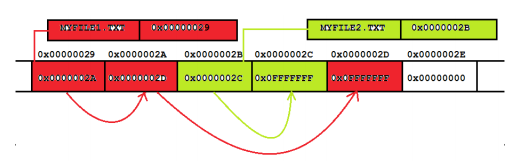
\includegraphics[scale=0.5]{figures/1.png}
	\caption{FAT32卷的FAT数据结构快照}
	\label{fig:2}
\end{figure}

\par
MYFILE1.TXT的第一个簇分配为0x00000029,针对该簇的FAT内容显示另一个簇0x0000002A,然后是0x0000002D,其FAT内容显示该簇是链中的最后一个簇。 类似地,对于MYFILE2.TXT,分配的第一个簇是0x0000002B,其FAT内容指向链中的下一个簇0x00000002C,这是其FAT内容指向的链中的最后一个簇。

\section{约束}
FAT32 FAT条目实际上使用低28位来寻址簇。 FAT32 FAT条目的高4位是保留的,只有在格式化卷时才会更改,此时整个32位FAT条目应归零,包括高4位。 这意味着所有这些32位群集条目值:0xA0000000,0xB0000000和0x00000000表示空闲群集,因为低28位设置为0。
\par
假设32位空闲簇值当前为0xA0000000,并且我们希望通过在其中存储值0x0FFFFFF7来将此簇标记为坏。 然后32位条目应包含值0xAFFFFFF7,因为当我们写入0x0FFFFFF7坏簇标记时,我们必须保留高4位。
\par
因为BPB在引导扇区的偏移11处指示的每个扇区的字节数总是可以被4整除,所以FAT32 FAT条目永远不会跨越扇区边界

\section{FAT中的前两个条目存储特殊值}
\begin{itemize}
	\item 第一个条目包含引导扇区偏移21处的BPB副本,该副本长度为8位,表示存储介质的类型。 此条目的高4和低8之间的剩余20位设置为1。
	\item 第二个条目存储EOC标记。 此条目的高位两位有时用于脏卷管理:如果设置为1则高位指示上次关闭是否干净,否则异常。 如果设置为1,则下一个最高位表示在上一次安装期间没有检测到磁盘I / O错误,否则有其他错误。
\end{itemize}

因为前两个FAT条目存储特殊值,所以没有簇0或1. FAT32 FAT数据结构中的第一个可寻址簇是簇2,这就是为什么引导扇区偏移44处的BPB值表示根目录簇的原因 number不能小于2,通常为2,即根目录位于文件/目录区域的开头。

\section{公式}
此处计算的所有扇区号都是相对于FAT32卷的第一个扇区,即引导扇区,并不一定直接映射到驱动器上,因为由于分区和代码,卷的扇区0不一定是驱动器的扇区0 片段采用CProgramming语言。
\par
文件/目录区域的开始,即集群2的第一个扇区,计算如下:
\begin{equation}
\begin{aligned}
FirstDataSector &= BPB\_ResvdSecCnt + (BPB\_NumFATs * FATSz)\\
&BPB\_ResvdSecCnt\ is \ the \ number \ of \ reserved\\
&sectors\ at \ offset\ 14\ of\ Boot\ sector\\
&BPB\_NumFATs\ is\ the\ count\ of\ FAT\ data\\
&structures\ at\ offset\ 16\ of\ Boot\ Sector\\
&FATSz\ is\ the\ count\ of\ sectors\ occupied\ by\ one\\
&FAT\ copy\ at\ offset\ 36\ of\ Boot\ Sector
\end{aligned}
\end{equation}

\par
给定任何有效的数据簇号N,该簇的第一扇区的扇区号计算如下:
\begin{equation}
\begin{aligned}
FirstSectorofCluster &= ((N – 2) *BPB\_SecPerClus) + FirstDataSector\\
&BPB\_SecPerClus\ is\ the\ count\ of\ sectors per\\
&cluster\ at\ offset\ 13\ of\ Boot\ Sector
\end{aligned}
\end{equation}

\par
给定任何有效数据簇号N,包含其条目的FAT扇区号和该FAT扇区中的偏移量计算如下:
\begin{equation}
\begin{aligned}
FATOffset &= N * 4\\
ThisFATSecNum &= BPB\_ResvdSecCnt +(FATOffset / BPB\_BytsPerSec)\\
ThisFATEntOffset &= FATOffset \%BPB\_BytsPerSec\\
&BPB\_BytsPerSec\ is\ the\ count\ of\ bytes\ per\ sector\\
&at\ offset\ 11\ of\ Boot\ Sector\\
\end{aligned}
\end{equation}

\par
上面计算的FAT扇区属于FAT的第一个副本; 如果要使用第二个副本,则FAT扇区计算如下:
\begin{equation}
ThisFATSecNum = BPB\_ResvdSecCnt +(FATOffset / BPB\_BytsPerSec)+ FATSz
\end{equation}













